% !TeX TXS-program:bibliography = txs:///biber
\documentclass[14pt, russian]{scrartcl}
\let\counterwithout\relax
\let\counterwithin\relax
%\usepackage{lmodern}
\usepackage{float}
\usepackage{xcolor}
\usepackage{extsizes}
\usepackage{subfig}
\usepackage[export]{adjustbox}
\usepackage{tocvsec2} % возможность менять учитываемую глубину разделов в оглавлении
\usepackage[subfigure]{tocloft}
\usepackage[newfloat]{minted}
\captionsetup[listing]{position=top}

\AtBeginEnvironment{figure}{\vspace{0.5cm}}
\AtBeginEnvironment{table}{\vspace{0.5cm}}
\AtBeginEnvironment{listing}{\vspace{0.5cm}}
\AtBeginEnvironment{algorithm}{\vspace{0.5cm}}
\AtBeginEnvironment{minted}{\vspace{-0.5cm}}

\usepackage{fancyvrb}
\usepackage{ulem,bm,mathrsfs,ifsym} %зачеркивания, особо жирный стиль и RSFS начертание
\usepackage{sectsty} % переопределение стилей подразделов
%%%%%%%%%%%%%%%%%%%%%%%

%%% Поля и разметка страницы %%%
\usepackage{pdflscape}                              % Для включения альбомных страниц
\usepackage{geometry}                               % Для последующего задания полей
\geometry{a4paper,tmargin=2cm,bmargin=2cm,lmargin=3cm,rmargin=1cm} % тоже самое, но лучше

%%% Математические пакеты %%%
\usepackage{amsthm,amsfonts,amsmath,amssymb,amscd}  % Математические дополнения от AMS
\usepackage{mathtools}                              % Добавляет окружение multlined
\usepackage[perpage]{footmisc}
%\usepackage{times}

%%%% Установки для размера шрифта 14 pt %%%%
%% Формирование переменных и констант для сравнения (один раз для всех подключаемых файлов)%%
%% должно располагаться до вызова пакета fontspec или polyglossia, потому что они сбивают его работу
%\newlength{\curtextsize}
%\newlength{\bigtextsize}
%\setlength{\bigtextsize}{13pt}
\KOMAoptions{fontsize=14pt}

\makeatletter
\def\showfontsize{\f@size{} point}
\makeatother

%\makeatletter
%\show\f@size                                       % неплохо для отслеживания, но вызывает стопорение процесса, если документ компилируется без команды  -interaction=nonstopmode 
%\setlength{\curtextsize}{\f@size pt}
%\makeatother

%шрифт times
\usepackage{tempora}
%\usepackage{pscyr}
%\setmainfont[Ligatures={TeX,Historic}]{Times New Roman}

   %%% Решение проблемы копирования текста в буфер кракозябрами
%    \input glyphtounicode.tex
%    \input glyphtounicode-cmr.tex %from pdfx package
%    \pdfgentounicode=1
    \usepackage{cmap}                               % Улучшенный поиск русских слов в полученном pdf-файле
    \usepackage[T1]{fontenc}                       % Поддержка русских букв
    \usepackage[utf8]{inputenc}                     % Кодировка utf8
    \usepackage[english, main=russian]{babel}            % Языки: русский, английский
%   \IfFileExists{pscyr.sty}{\usepackage{pscyr}}{}  % Красивые русские шрифты
%\renewcommand{\rmdefault}{ftm}
%%% Оформление абзацев %%%
\usepackage{indentfirst}                            % Красная строка
%\usepackage{eskdpz}

%%% Таблицы %%%
\usepackage{longtable}                              % Длинные таблицы
\usepackage{multirow,makecell,array}                % Улучшенное форматирование таблиц
\usepackage{booktabs}                               % Возможность оформления таблиц в классическом книжном стиле (при правильном использовании не противоречит ГОСТ)

%%% Общее форматирование
\usepackage{soulutf8}                               % Поддержка переносоустойчивых подчёркиваний и зачёркиваний
\usepackage{icomma}                                 % Запятая в десятичных дробях



%%% Изображения %%%
\usepackage{graphicx}                               % Подключаем пакет работы с графикой
\usepackage{wrapfig}

%%% Списки %%%
\usepackage{enumitem}

%%% Подписи %%%
\usepackage{caption}                                % Для управления подписями (рисунков и таблиц) % Может управлять номерами рисунков и таблиц с caption %Иногда может управлять заголовками в списках рисунков и таблиц
%% Использование:
%\begin{table}[h!]\ContinuedFloat - чтобы не переключать счетчик
%\captionsetup{labelformat=continued}% должен стоять до самого caption
%\caption{}
% либо ручками \caption*{Продолжение таблицы~\ref{...}.} :)

%%% Интервалы %%%
\addto\captionsrussian{%
  \renewcommand{\listingname}{Листинг}%
}
%%% Счётчики %%%
\usepackage[figure,table,section]{totalcount}               % Счётчик рисунков и таблиц
\DeclareTotalCounter{lstlisting}
\usepackage{totcount}                               % Пакет создания счётчиков на основе последнего номера подсчитываемого элемента (может требовать дважды компилировать документ)
\usepackage{totpages}                               % Счётчик страниц, совместимый с hyperref (ссылается на номер последней страницы). Желательно ставить последним пакетом в преамбуле

%%% Продвинутое управление групповыми ссылками (пока только формулами) %%%
%% Кодировки и шрифты %%%

%   \newfontfamily{\cyrillicfont}{Times New Roman}
%   \newfontfamily{\cyrillicfonttt}{CMU Typewriter Text}
	%\setmainfont{Times New Roman}
	%\newfontfamily\cyrillicfont{Times New Roman}
	%\setsansfont{Times New Roman}                    %% задаёт шрифт без засечек
%	\setmonofont{Liberation Mono}               %% задаёт моноширинный шрифт
%    \IfFileExists{pscyr.sty}{\renewcommand{\rmdefault}{ftm}}{}
%%% Интервалы %%%
%linespread-реализация ближе к реализации полуторного интервала в ворде.
%setspace реализация заточена под шрифты 10, 11, 12pt, под остальные кегли хуже, но всё же ближе к типографской классике. 
\linespread{1.3}                    % Полуторный интервал (ГОСТ Р 7.0.11-2011, 5.3.6)
%\renewcommand{\@biblabel}[1]{#1}

%%% Гиперссылки %%%
\usepackage{hyperref}

%%% Выравнивание и переносы %%%
\sloppy                             % Избавляемся от переполнений
\clubpenalty=10000                  % Запрещаем разрыв страницы после первой строки абзаца
\widowpenalty=10000                 % Запрещаем разрыв страницы после последней строки абзаца

\makeatletter % малые заглавные, small caps shape
\let\@@scshape=\scshape
\renewcommand{\scshape}{%
  \ifnum\strcmp{\f@series}{bx}=\z@
    \usefont{T1}{cmr}{bx}{sc}%
  \else
    \ifnum\strcmp{\f@shape}{it}=\z@
      \fontshape{scsl}\selectfont
    \else
      \@@scshape
    \fi
  \fi}
\makeatother

%%% Подписи %%%
%\captionsetup{%
%singlelinecheck=off,                % Многострочные подписи, например у таблиц
%skip=2pt,                           % Вертикальная отбивка между подписью и содержимым рисунка или таблицы определяется ключом
%justification=centering,            % Центрирование подписей, заданных командой \caption
%}
%%%        Подключение пакетов                 %%%
\usepackage{ifthen}                 % добавляет ifthenelse
%%% Инициализирование переменных, не трогать!  %%%
\newcounter{intvl}
\newcounter{otstup}
\newcounter{contnumeq}
\newcounter{contnumfig}
\newcounter{contnumtab}
\newcounter{pgnum}
\newcounter{bibliosel}
\newcounter{chapstyle}
\newcounter{headingdelim}
\newcounter{headingalign}
\newcounter{headingsize}
\newcounter{tabcap}
\newcounter{tablaba}
\newcounter{tabtita}
%%%%%%%%%%%%%%%%%%%%%%%%%%%%%%%%%%%%%%%%%%%%%%%%%%

%%% Область упрощённого управления оформлением %%%

%% Интервал между заголовками и между заголовком и текстом
% Заголовки отделяют от текста сверху и снизу тремя интервалами (ГОСТ Р 7.0.11-2011, 5.3.5)
\setcounter{intvl}{3}               % Коэффициент кратности к размеру шрифта

%% Отступы у заголовков в тексте
\setcounter{otstup}{0}              % 0 --- без отступа; 1 --- абзацный отступ

%% Нумерация формул, таблиц и рисунков
\setcounter{contnumeq}{1}           % Нумерация формул: 0 --- пораздельно (во введении подряд, без номера раздела); 1 --- сквозная нумерация по всей диссертации
\setcounter{contnumfig}{1}          % Нумерация рисунков: 0 --- пораздельно (во введении подряд, без номера раздела); 1 --- сквозная нумерация по всей диссертации
\setcounter{contnumtab}{1}          % Нумерация таблиц: 0 --- пораздельно (во введении подряд, без номера раздела); 1 --- сквозная нумерация по всей диссертации

%% Оглавление
\setcounter{pgnum}{0}               % 0 --- номера страниц никак не обозначены; 1 --- Стр. над номерами страниц (дважды компилировать после изменения)

%% Библиография
\setcounter{bibliosel}{1}           % 0 --- встроенная реализация с загрузкой файла через движок bibtex8; 1 --- реализация пакетом biblatex через движок biber

%% Текст и форматирование заголовков
\setcounter{chapstyle}{1}           % 0 --- разделы только под номером; 1 --- разделы с названием "Глава" перед номером
\setcounter{headingdelim}{1}        % 0 --- номер отделен пропуском в 1em или \quad; 1 --- номера разделов и приложений отделены точкой с пробелом, подразделы пропуском без точки; 2 --- номера разделов, подразделов и приложений отделены точкой с пробелом.

%% Выравнивание заголовков в тексте
\setcounter{headingalign}{0}        % 0 --- по центру; 1 --- по левому краю

%% Размеры заголовков в тексте
\setcounter{headingsize}{0}         % 0 --- по ГОСТ, все всегда 14 пт; 1 --- пропорционально изменяющийся размер в зависимости от базового шрифта

%% Подпись таблиц
\setcounter{tabcap}{0}              % 0 --- по ГОСТ, номер таблицы и название разделены тире, выровнены по левому краю, при необходимости на нескольких строках; 1 --- подпись таблицы не по ГОСТ, на двух и более строках, дальнейшие настройки: 
%Выравнивание первой строки, с подписью и номером
\setcounter{tablaba}{2}             % 0 --- по левому краю; 1 --- по центру; 2 --- по правому краю
%Выравнивание строк с самим названием таблицы
\setcounter{tabtita}{1}             % 0 --- по левому краю; 1 --- по центру; 2 --- по правому краю

%%% Рисунки %%%
\DeclareCaptionLabelSeparator*{emdash}{~--- }             % (ГОСТ 2.105, 4.3.1)
\captionsetup[figure]{labelsep=emdash,font=onehalfspacing,position=bottom}

%%% Таблицы %%%
\ifthenelse{\equal{\thetabcap}{0}}{%
    \newcommand{\tabcapalign}{\raggedright}  % по левому краю страницы или аналога parbox
}

\ifthenelse{\equal{\thetablaba}{0} \AND \equal{\thetabcap}{1}}{%
    \newcommand{\tabcapalign}{\raggedright}  % по левому краю страницы или аналога parbox
}

\ifthenelse{\equal{\thetablaba}{1} \AND \equal{\thetabcap}{1}}{%
    \newcommand{\tabcapalign}{\centering}    % по центру страницы или аналога parbox
}

\ifthenelse{\equal{\thetablaba}{2} \AND \equal{\thetabcap}{1}}{%
    \newcommand{\tabcapalign}{\raggedleft}   % по правому краю страницы или аналога parbox
}

\ifthenelse{\equal{\thetabtita}{0} \AND \equal{\thetabcap}{1}}{%
    \newcommand{\tabtitalign}{\raggedright}  % по левому краю страницы или аналога parbox
}

\ifthenelse{\equal{\thetabtita}{1} \AND \equal{\thetabcap}{1}}{%
    \newcommand{\tabtitalign}{\centering}    % по центру страницы или аналога parbox
}

\ifthenelse{\equal{\thetabtita}{2} \AND \equal{\thetabcap}{1}}{%
    \newcommand{\tabtitalign}{\raggedleft}   % по правому краю страницы или аналога parbox
}

\DeclareCaptionFormat{tablenocaption}{\tabcapalign #1\strut}        % Наименование таблицы отсутствует
\ifthenelse{\equal{\thetabcap}{0}}{%
    \DeclareCaptionFormat{tablecaption}{\tabcapalign #1#2#3}
    \captionsetup[table]{labelsep=emdash}                       % тире как разделитель идентификатора с номером от наименования
}{%
    \DeclareCaptionFormat{tablecaption}{\tabcapalign #1#2\par%  % Идентификатор таблицы на отдельной строке
        \tabtitalign{#3}}                                       % Наименование таблицы строкой ниже
    \captionsetup[table]{labelsep=space}                        % пробельный разделитель идентификатора с номером от наименования
}
\captionsetup[table]{format=tablecaption,singlelinecheck=off,font=onehalfspacing,position=top,skip=-5pt}  % многострочные наименования и прочее
\DeclareCaptionLabelFormat{continued}{Продолжение таблицы~#2}
\setlength{\belowcaptionskip}{.2cm}
\setlength{\intextsep}{0ex}

%%% Подписи подрисунков %%%
\renewcommand{\thesubfigure}{\asbuk{subfigure}}           % Буквенные номера подрисунков
\captionsetup[subfigure]{font={normalsize},               % Шрифт подписи названий подрисунков (не отличается от основного)
    labelformat=brace,                                    % Формат обозначения подрисунка
    justification=centering,                              % Выключка подписей (форматирование), один из вариантов            
}
%\DeclareCaptionFont{font12pt}{\fontsize{12pt}{13pt}\selectfont} % объявляем шрифт 12pt для использования в подписях, тут же надо интерлиньяж объявлять, если не наследуется
%\captionsetup[subfigure]{font={font12pt}}                 % Шрифт подписи названий подрисунков (всегда 12pt)

%%% Настройки гиперссылок %%%

\definecolor{linkcolor}{rgb}{0.0,0,0}
\definecolor{citecolor}{rgb}{0,0.0,0}
\definecolor{urlcolor}{rgb}{0,0,0}

\hypersetup{
    linktocpage=true,           % ссылки с номера страницы в оглавлении, списке таблиц и списке рисунков
%    linktoc=all,                % both the section and page part are links
%    pdfpagelabels=false,        % set PDF page labels (true|false)
    plainpages=true,           % Forces page anchors to be named by the Arabic form  of the page number, rather than the formatted form
    colorlinks,                 % ссылки отображаются раскрашенным текстом, а не раскрашенным прямоугольником, вокруг текста
    linkcolor={linkcolor},      % цвет ссылок типа ref, eqref и подобных
    citecolor={citecolor},      % цвет ссылок-цитат
    urlcolor={urlcolor},        % цвет гиперссылок
    pdflang={ru},
}
\urlstyle{same}
%%% Шаблон %%%
%\DeclareRobustCommand{\todo}{\textcolor{red}}       % решаем проблему превращения названия цвета в результате \MakeUppercase, http://tex.stackexchange.com/a/187930/79756 , \DeclareRobustCommand protects \todo from expanding inside \MakeUppercase
\setlength{\parindent}{2.5em}                       % Абзацный отступ. Должен быть одинаковым по всему тексту и равен пяти знакам (ГОСТ Р 7.0.11-2011, 5.3.7).

%%% Списки %%%
% Используем дефис для ненумерованных списков (ГОСТ 2.105-95, 4.1.7)
%\renewcommand{\labelitemi}{\normalfont\bfseries~{---}} 
\renewcommand{\labelitemi}{\bfseries~{---}} 
\setlist{nosep,%                                    % Единый стиль для всех списков (пакет enumitem), без дополнительных интервалов.
    labelindent=\parindent,leftmargin=*%            % Каждый пункт, подпункт и перечисление записывают с абзацного отступа (ГОСТ 2.105-95, 4.1.8)
}
%%%%%%%%%%%%%%%%%%%%%%
%\usepackage{xltxtra} % load xunicode

\usepackage{ragged2e}
\usepackage[explicit]{titlesec}
\usepackage{placeins}
\usepackage{xparse}
\usepackage{csquotes}

\usepackage{listingsutf8}
\usepackage{url} %пакеты расширений
\usepackage{algorithm, algorithmicx}
\usepackage[noend]{algpseudocode}
\usepackage{blkarray}
\usepackage{chngcntr}
\usepackage{tabularx}
\usepackage[backend=biber, 
    bibstyle=gost-numeric,
    citestyle=nature]{biblatex}
\newcommand*\template[1]{\text{<}#1\text{>}}
\addbibresource{biblio.bib}
  
\titleformat{name=\section,numberless}[block]{\normalfont\Large\centering}{}{0em}{#1}
\titleformat{\section}[block]{\normalfont\Large\bfseries\raggedright}{}{0em}{\thesection\hspace{0.25em}#1}
\titleformat{\subsection}[block]{\normalfont\Large\bfseries\raggedright}{}{0em}{\thesubsection\hspace{0.25em}#1}
\titleformat{\subsubsection}[block]{\normalfont\large\bfseries\raggedright}{}{0em}{\thesubsubsection\hspace{0.25em}#1}

\let\Algorithm\algorithm
\renewcommand\algorithm[1][]{\Algorithm[#1]\setstretch{1.5}}
%\renewcommand{\listingscaption}{Листинг}

\usepackage{pifont}
\usepackage{calc}
\usepackage{suffix}
\usepackage{csquotes}
\DeclareQuoteStyle{russian}
    {\guillemotleft}{\guillemotright}[0.025em]
    {\quotedblbase}{\textquotedblleft}
\ExecuteQuoteOptions{style=russian}
\newcommand{\enq}[1]{\enquote{#1}}  
\newcommand{\eng}[1]{\begin{english}#1\end{english}}
% Подчиненные счетчики в окружениях http://old.kpfu.ru/journals/izv_vuz/arch/sample1251.tex
\newcounter{cTheorem} 
\newcounter{cDefinition}
\newcounter{cConsequent}
\newcounter{cExample}
\newcounter{cLemma}
\newcounter{cConjecture}
\newtheorem{Theorem}{Теорема}[cTheorem]
\newtheorem{Definition}{Определение}[cDefinition]
\newtheorem{Consequent}{Следствие}[cConsequent]
\newtheorem{Example}{Пример}[cExample]
\newtheorem{Lemma}{Лемма}[cLemma]
\newtheorem{Conjecture}{Гипотеза}[cConjecture]

\renewcommand{\theTheorem}{\arabic{Theorem}}
\renewcommand{\theDefinition}{\arabic{Definition}}
\renewcommand{\theConsequent}{\arabic{Consequent}}
\renewcommand{\theExample}{\arabic{Example}}
\renewcommand{\theLemma}{\arabic{Lemma}}
\renewcommand{\theConjecture}{\arabic{Conjecture}}
%\makeatletter
\NewDocumentCommand{\Newline}{}{\text{\\}}
\newcommand{\sequence}[2]{\ensuremath \left(#1,\ \dots,\ #2\right)}

\definecolor{mygreen}{rgb}{0,0.6,0}
\definecolor{mygray}{rgb}{0.5,0.5,0.5}
\definecolor{mymauve}{rgb}{0.58,0,0.82}
\renewcommand{\listalgorithmname}{Список алгоритмов}
\floatname{algorithm}{Листинг}
\renewcommand{\lstlistingname}{Листинг}
\renewcommand{\thealgorithm}{\arabic{algorithm}}

\newcommand{\refAlgo}[1]{(листинг \ref{#1})}
\newcommand{\refImage}[1]{(рисунок \ref{#1})}

\renewcommand{\theenumi}{\arabic{enumi}.}% Меняем везде перечисления на цифра.цифра	
\renewcommand{\labelenumi}{\arabic{enumi}.}% Меняем везде перечисления на цифра.цифра
\renewcommand{\theenumii}{\arabic{enumii}}% Меняем везде перечисления на цифра.цифра
\renewcommand{\labelenumii}{(\arabic{enumii})}% Меняем везде перечисления на цифра.цифра
\renewcommand{\theenumiii}{\roman{enumiii}}% Меняем везде перечисления на цифра.цифра
\renewcommand{\labelenumiii}{(\roman{enumiii})}% Меняем везде перечисления на цифра.цифра
%\newfontfamily\AnkaCoder[Path=src/fonts/]{AnkaCoder-r.ttf}
\renewcommand{\labelitemi}{---}
\renewcommand{\labelitemii}{---}

%\usepackage{courier}

\lstdefinelanguage{Refal}{
  alsodigit = {.,<,>},
  morekeywords = [1]{$ENTRY},
  morekeywords = [2]{Go, Put, Get, Open, Close, Arg, Add, Sub, Mul, Div, Symb, Explode, Implode},
  %keyword4
  morekeywords = [3]{<,>},
  %keyword5
  morekeywords = [4]{e.,t.,s.},
  sensitive = true,
  morecomment = [l]{*},
  morecomment = [s]{/*}{*/},
  commentstyle = \color{mygreen},
  morestring = [b]",
  morestring = [b]',
  stringstyle = \color{purple}
}

\makeatletter
\def\p@subsection{}
\def\p@subsubsection{\thesection\,\thesubsection\,}
\makeatother
\newcommand{\prog}[1]{{\ttfamily\small#1}}
\lstset{ %
  backgroundcolor=\color{white},   % choose the background color; you must add \usepackage{color} or \usepackage{xcolor}
  basicstyle=\ttfamily\footnotesize, 
  %basicstyle=\footnotesize\AnkaCoder,        % the size of the fonts that are used for the code
  breakatwhitespace=false,         % sets if automatic breaks shoulbd only happen at whitespace
  breaklines=true,                 % sets automatic line breaking
  captionpos=top,                    % sets the caption-position to bottom
  commentstyle=\color{mygreen},    % comment style
  deletekeywords={...},            % if you want to delete keywords from the given language
  escapeinside={\%*}{*)},          % if you want to add LaTeX within your code
  extendedchars=true,              % lets you use non-ASCII characters; for 8-bits encodings only, does not work with UTF-8
  inputencoding=utf8,
  frame=single,                    % adds a frame around the code
  keepspaces=true,                 % keeps spaces in text, useful for keeping indentation of code (possibly needs columns=flexible)
  keywordstyle=\bf,       % keyword style
  language=Refal,                    % the language of the code
  morekeywords={<,>,$ENTRY,Go,Arg, Open, Close, e., s., t., Get, Put}, 
  							       % if you want to add more keywords to the set
  numbers=left,                    % where to put the line-numbers; possible values are (none, left, right)
  numbersep=5pt,                   % how far the line-numbers are from the code
  xleftmargin=25pt,
  xrightmargin=25pt,
  numberstyle=\small\color{black}, % the style that is used for the line-numbers
  rulecolor=\color{black},         % if not set, the frame-color may be changed on line-breaks within not-black text (e.g. comments (green here))
  showspaces=false,                % show spaces everywhere adding particular underscores; it overrides 'showstringspaces'
  showstringspaces=false,          % underline spaces within strings only
  showtabs=false,                  % show tabs within strings adding particular underscores
  stepnumber=1,                    % the step between two line-numbers. If it's 1, each line will be numbered
  stringstyle=\color{mymauve},     % string literal style
  tabsize=8,                       % sets default tabsize to 8 spaces
  title=\lstname                   % show the filename of files included with \lstinputlisting; also try caption instead of title
}
\newcommand{\anonsection}[1]{\cleardoublepage
\phantomsection
\addcontentsline{toc}{section}{\protect\numberline{}#1}
\section*{#1}\vspace*{2.5ex} % По госту положены 3 пустые строки после заголовка ненумеруемого раздела
}
\newcommand{\sectionbreak}{\clearpage}
\renewcommand{\sectionfont}{\normalsize} % Сбиваем стиль оглавления в стандартный
\renewcommand{\cftsecleader}{\cftdotfill{\cftdotsep}} % Точки в оглавлении напротив разделов

\renewcommand{\cftsecfont}{\normalfont\large} % Переключение на times в содержании
\renewcommand{\cftsubsecfont}{\normalfont\large} % Переключение на times в содержании

\usepackage{caption} 
%\captionsetup[table]{justification=raggedleft} 
%\captionsetup[figure]{justification=centering,labelsep=endash}
\usepackage{amsmath}    % \bar    (матрицы и проч. ...)
\usepackage{amsfonts}   % \mathbb (символ для множества действительных чисел и проч. ...)
\usepackage{mathtools}  % \abs, \norm
    \DeclarePairedDelimiter\abs{\lvert}{\rvert} % операция модуля
    \DeclarePairedDelimiter\norm{\lVert}{\rVert} % операция нормы
\DeclareTextCommandDefault{\textvisiblespace}{%
  \mbox{\kern.06em\vrule \@height.3ex}%
  \vbox{\hrule \@width.3em}%
  \hbox{\vrule \@height.3ex}}    
\newsavebox{\spacebox}
\begin{lrbox}{\spacebox}
\verb*! !
\end{lrbox}
\newcommand{\aspace}{\usebox{\spacebox}}
\DeclareTotalCounter{listing}

\makeatletter
\renewcommand*{\p@subsubsection}{}
\makeatother

\newcommand{\code}[1]{\texttt{#1}}
    
\begin{document}
\sloppy

\def\figurename{Рисунок}

\begin{titlepage}
	\thispagestyle{empty}
	\newpage

	\vspace*{-30pt}
	\hspace{-45pt}
	\begin{minipage}{0.17\textwidth}
		\hspace*{-20pt}\centering
		\includegraphics[width=1.3\textwidth]{emblem.png}
	\end{minipage}
	\begin{minipage}{0.82\textwidth}\small \textbf{
			\vspace*{-0.7ex}
			\hspace*{-10pt}\centerline{Министерство науки и высшего образования Российской Федерации}
			\vspace*{-0.7ex}
			\centerline{Федеральное государственное бюджетное образовательное учреждение }
			\vspace*{-0.7ex}
			\centerline{высшего образования}
			\vspace*{-0.7ex}
			\centerline{<<Московский государственный технический университет}
			\vspace*{-0.7ex}
			\centerline{имени Н.Э. Баумана}
			\vspace*{-0.7ex}
			\centerline{(национальный исследовательский университет)>>}
			\vspace*{-0.7ex}
			\centerline{(МГТУ им. Н.Э. Баумана)}}
	\end{minipage}

	\vspace{-2pt}
	\hspace{-34.5pt}\rule{\textwidth}{2.5pt}

	\vspace*{-20.3pt}
	\hspace{-34.5pt}\rule{\textwidth}{0.4pt}

	\vspace{0.5ex}
	\noindent \small ФАКУЛЬТЕТ\hspace{80pt} <<Информатика и системы управления>>

	\vspace*{-16pt}
	\hspace{35pt}\rule{0.855\textwidth}{0.4pt}

	\vspace{0.5ex}
	\noindent \small КАФЕДРА\hspace{50pt} <<Теоретическая информатика и компьютерные технологии>>

	\vspace*{-16pt}
	\hspace{25pt}\rule{0.875\textwidth}{0.4pt}


	\vspace{3em}

	\begin{center}
		\Large \bf{РАСЧЕТНО-ПОЯСНИТЕЛЬНАЯ ЗАПИСКА\\\textbf{\textit{К КУРСОВОЙ РАБОТЕ\\НА ТЕМУ:}} \\}
	\end{center}

	\vspace*{-6ex}
	\begin{center}
		\Large{\textit{\textbf{<<Разработка библиотеки для отслеживания }}}

		\vspace*{-3ex}
		\rule{0.9\textwidth}{1.2pt}

		\vspace*{-0.2ex}
		\Large{\textit{\textbf{событий файловой системы>>}}}
		\vspace*{-3ex}
		\vspace*{-0.2ex}
		\rule{0.9\textwidth}{1.2pt}

		\vspace*{-0.2ex}
		\rule{0.9\textwidth}{1.2pt}

		\vspace*{-0.2ex}
		\rule{0.9\textwidth}{1.2pt}

		\vspace*{-0.2ex}
		\rule{0.9\textwidth}{1.2pt}
	\end{center}

	\vspace{\fill}


	\newlength{\ML}
	\settowidth{\ML}{«\underline{\hspace{0.7cm}}» \underline{\hspace{2cm}}}

	\noindent Студент \underline{\text{ИУ9-51Б}} \hfill \underline{ \hspace{4cm}}\quad
	\underline{\raisebox{0.5ex}{\parbox{4cm}{\centering Старовойтов А.И.}}}

	\vspace{-2.1ex}
	\noindent\hspace{9ex}\scriptsize{(Группа)}\normalsize\hspace{170pt}\hspace{2ex}\scriptsize{(Подпись, дата)}\normalsize\hspace{30pt}\hspace{6ex}\scriptsize{(И.О. Фамилия)}\normalsize

	\bigskip

	\noindent Руководитель  \hfill \underline{\hspace{4cm}}\quad
	\underline{\raisebox{0.25ex}{\parbox{4cm}{\centering Вишняков И.Э.}}}

	\vspace{-2ex}
	\noindent\hspace{13.5ex}\normalsize\hspace{170pt}\hspace{2ex}\scriptsize{(Подпись, дата)}\normalsize\hspace{30pt}\hspace{6ex}\scriptsize{(И.О. Фамилия)}\normalsize

	\bigskip

	\noindent Консультант\hfill \underline{\hspace{4cm}}\quad
	\underline{\hspace{4cm}}

	\vspace{-2ex}
	\noindent\hspace{13.5ex}\normalsize\hspace{170pt}\hspace{2ex}\scriptsize{(Подпись, дата)}\normalsize\hspace{30pt}\hspace{6ex}\scriptsize{(И.О. Фамилия)}\normalsize
	\vfill

	%\vspace{\fill}



	\begin{center}
		\textsl{2023 г.}
	\end{center}
\end{titlepage}

%\renewcommand{\ttdefault}{pcr}

\setlength{\tabcolsep}{3pt}
\newpage
\setcounter{page}{2}
%----------------------------------------------------------------------------
%                  ОТСЮДА --- СОБСТВЕННО ТЕКСТ
%----------------------------------------------------------------------------

\newpage
\renewcommand\contentsname{\hfill{\normalfont{СОДЕРЖАНИЕ}}\hfill}  %Оглавление
\tableofcontents
\newpage
\anonsection{ВВЕДЕНИЕ}  %Введение

Отслеживание событий файловой системы применяется в различных видах программного
обеспечения, начиная от системных служб, заканчивая десктопными приложениями.
Это подразумевает получение информации об операциях, променяемых к файлам и
каталогам, в реальном времени.

Уже долгое время, операционная система Linux лидирует в сегменте серверов и
мобильных устройств. Современный API Linux предоставляет набор системных вызовов
inotify, который позволяет отслеживать события файловой системы.

В то же время, язык программирования Go стремительно набирает популярность, как
инструмент разработки серверных приложений. Хотя Go реализует системные вызовы
inotify, до сих пор не существет библиотеки, реализующей необходимые абстракции
и предоставляющей удобный интерфейс для отслеживания событий файловой системы.

Целью данной курсовой работы является разработка библиотеки на языке
программирования Go для отслеживания событий файловой системы. Библиотека должна
скрывать детали использования системных вызовов inotify и предоставлять удобный
интерфейс, не ограничивающий возможности пользователя.

\section{Обзор предметной области}

Примерами приложений, которые используют отслеживание событий файловой системы
являются:

\begin{itemize}
  \item Графический файловый менеджер. Использует события для отображения
        актуального состояния каталога.
  \item Системы текстового поиска по файлам или поиска самих файлов. Используют
        события файловой системы для поддержания поискового индекса.
  \item Любые системные службы и пользовательские приложения, демоны, которые в
        реальном времени отслеживают изменения в конфигурационных файлах.
  \item Системы сборки и анализа программного кода, интегрированные среды
        разработки. Отслеживают изменения в файлах исходного кода для последущей
        сборки или анализа.
  \item Антивирусы. На основе событий принимают решения по разрешению или
        запрещению определенных операций над файлами.
\end{itemize}

Примером приложения, которое использует отслеживание событий файловой системы,
может быть графический файловый менеджер. Он использует информацию об операциях
над файловой системой, таких как удаление или создание файлов или каталогов,
для обновления графического интерфейса. Другим примером могут являться системные
службы (демоны), которым необходимо отслеживать изменения в файлах конфигурации.

Простейший способ отслеживать события файловой системы --- это периодическое
рекурсивное чтение с одновременным сравнением с предыдущей закэшированной
версией. Этот метод не требует специальной поддержки со стороны операционной
системы, но влечет за собой высокие накладные расходы и вероятность пропустить
некоторые события. Кроме того, некоторые виды событий, таких как переименование
файла, трудно отслеживать таким способом. Однако, на данный момент это
единственный способ отслеживать события в удаленных (сетевых) файловых системах.

Начиная с версии 2.4, в ядре Linux существует механизм под названием <<dnotify>>
\cite{kerrisk2010linux}, который предоставляет уведомления об операциях над
файлами при помощи сигналов.

\subsection{Механизм dnotify}

dnotify предоставляет уведомления об операциях над файловой системой с помощью
сигналов, что усложняет разработку приложения, особенно на таком высокоуровневом
языке, как Go. Кроме того, затруднено применение этого механизма в библиотеках,
так как пользовательский код может переопределять обработчики нужных сигналов,
что нельзя ограничить другим способом, кроме запрета в документации.

Минимальная единица, уведомления об операциях над которой можно получать
уведомления --- каталог. При этом приложение будет также получать уведомления
об операциях над файлами внутри этого каталога, но не рекурсивно.

Для того, чтобы подписаться на обновления каталога с помощью dnotify, приложение
должно открыть для нее файловый дескриптор. Это влечет за собой две проблемы:

\begin{itemize}
  \item открытый файловый дескриптор блокирует отключение (размонтирование)
        файловой системы от иерархического дерева каталогов;
  \item так как для отслеживания событий для каждого каталога открывается новый
        файловый дескриптор, это может привести к их большому потреблению.
\end{itemize}

Когда происходит изменение файла в отслеживаемом каталоге, dnotify сообщает, что
такое событие произошло, но не предоставляет информации, какой именно файл
изменен. Это позволяет избежать периодического чтения содержимого каталога, но
не избавляет от необходимости кешировать информацию о файлах в каталоге.

\subsection{Механизм inotify}%
\label{subsec:inotify}

Начиная с версии 2.6.13 ядро Linux предоставляет механизм для отслеживания
событий файловой системы под названием <<inotify>> \cite{inotify}. Этот интерфейс полностью
заменил dnotify, расширив его возможности и гибкость.

Inotify можно использовать для мониторинга отдельных файлов или каталогов. Когда
отслеживается каталог, Механизм предоставляет события для самого каталога и для
файлов внутри каталога.

Основные преимущества inotify над dnotify:

\begin{itemize}
  \item inotify не использует сигналы для уведомления программы о событиях.
  \item inotify может отслеживать события каталога или отдельного файла.
  \item inotify предоставляет больше информации о событиях, а так же относительно каких
        файлов они происходят.
  \item В некоторых ситуациях inotify более надежен, чем dnotify.
\end{itemize}

Ограничения inotify:

\begin{itemize}
  \item Дублирующие одинаковые события сбрасываются, если еще не были прочитаны.
        Поэтому, нельзя использовать механизм inotify для подсчета событий
        файловой системы.
  \item Потребление памяти линейно зависит от количества отслеживаемых
        каталогов.
  \item Не предоствляется информация о пользователе или процессе, которые
        совершили операцию, вызвавшую отправку события.
  \item Не поддерживаются события удаленных (сетевых) файловых систем и
        некоторых псевдо-файловых систем, таких как /proc, /sys, /dev/pts и так
        далее.
  \item Изменения файлов через mmap, msync и munmap не генерируют события.
  \item Файлы, к которым относятся события, идентифицируются по названию.
        Значит, к моменту когда приложение будет обрабатывать событие, искомый
        файл уже может быть переименован или удален.
  \item Отслеживание событий применяется к каталогам нерекурсивно.
  \item Очередь событий в ядре может быть переполнена. В этом случае новые
        события теряются.
  \item Интерфейс inotify идентифицирует события с помощью дескрипторов
        отслеживания. Ответственность за кэширование сопоставления (если оно
        необходимо) между дескрипторами отслеживания и путями к ним лежит на
        пользовательском коде. Стоит учитывать, что переименования каталогов
        могут повлиять на несколько путей в кэше.
  \item Если отслеживается все поддерево каталога и в этом дереве создается
        новый подкаталог или существующий каталог переименовывается в это
        дерево, может возникнуть ситуация, когда пользовательский код еще не
        настроил отслеживание событий нового каталога, файлы (и подкаталоги)
        могут уже появиться внутри подкаталога. Решением будет являться
        сканирование содержимого подкаталога сразу после добавления в списо
        отслеживаемых.
\end{itemize}

Основной сценарий использования механизма inotify --- эффективный мониторинг и
кэширования состояния набора объектов файловой системы \cite{linuxmagazine}. Этот сценарий используют
системы сборки и анализа кода \cite{tup}, системы поиска по файлам и многие другие. Однако,
разработчики пользовательских приложений должны учитывать тот факт, что ошибки в
логике мониторинга или гонки, описанные в ограничениях выше, могут привести к
несоответствию кэша и состояния файловой системы. Поэтому, разумно реализовать
некоторую периодическую проверку согласованности, и перестраивать кэш при
обнаружении несоответствий. Например, перестраивать кэш необходимо и при
переполнении очереди событий.

Ядро операционной системы Linux предоставляет следующие функции в рамках
интерфейса inotify:

\begin{enumerate}
  \item \code{inotify\_init} и \code{inotify\_init1};
  \item \code{inotify\_add\_watch};
  \item \code{inotify\_rm\_watch};
  \item \code{read} и \code{close} применимо к файловым дескрипторам inotify.
\end{enumerate}

Далее приводятся шаги, необходимые для использования механизма inotify:

\begin{enumerate}
  \item Приложение использует \code{inotify\_init()} для создания экземпляра
        inotify. Этот системный вызов возвращает файловый дескриптор, который
        является ссылкой на экземпляр inotify для использования в последующих
        вызовах.
  \item Приложение информирует ядро о том, события по каким файлам и каталогам
        представляют интерес, используя функцию \code{inotify\_add\_watch()} для
        добавления элементов в список наблюдения экземпляра inotify, созданного
        на предыдущем шаге. Каждый элемент наблюдения состоит из имени пути и
        соответствующей битовой маски. Битовая маска определяет набор событий,
        которые будут отслеживаться для имени пути. Схема объекта представлена
        на рисунке \ref{fig:inotify_object}. В качестве результата функция
        \code{inotify\_add\_watch()} возвращает дескриптор наблюдения, который
        используется для ссылки на экзепмляр наблюдения в последующих операциях.
        (Системный вызов \code{inotify\_rm\_watch()} выполняет обратную задачу,
        удаляя экземпляр наблюдения, который ранее был добавлен в экземпляр
        inotify.)
  \item Чтобы получать уведомления о событиях, приложение делает вызовы
        \code{read()} с файловым дескриптором inotify. Каждый успешный
        \code{read()} возвращает одну или несколько структур inotify\_event,
        каждая из которых содержит информацию о событии, произошедшем с одним из
        путей, отслеживаемых с помощью этого экземпляра inotify.
  \item Когда приложение хочет завершить отслеживание событий, оно закрывает
        файловый дескриптор inotify. При этом автоматически удаляются все
        экземпляры наблюдения, связанные с экземпляром inotify.
\end{enumerate}

\begin{figure}[H]
  \centering
  \begin{minipage}[t]{.9\textwidth}
    \centering
    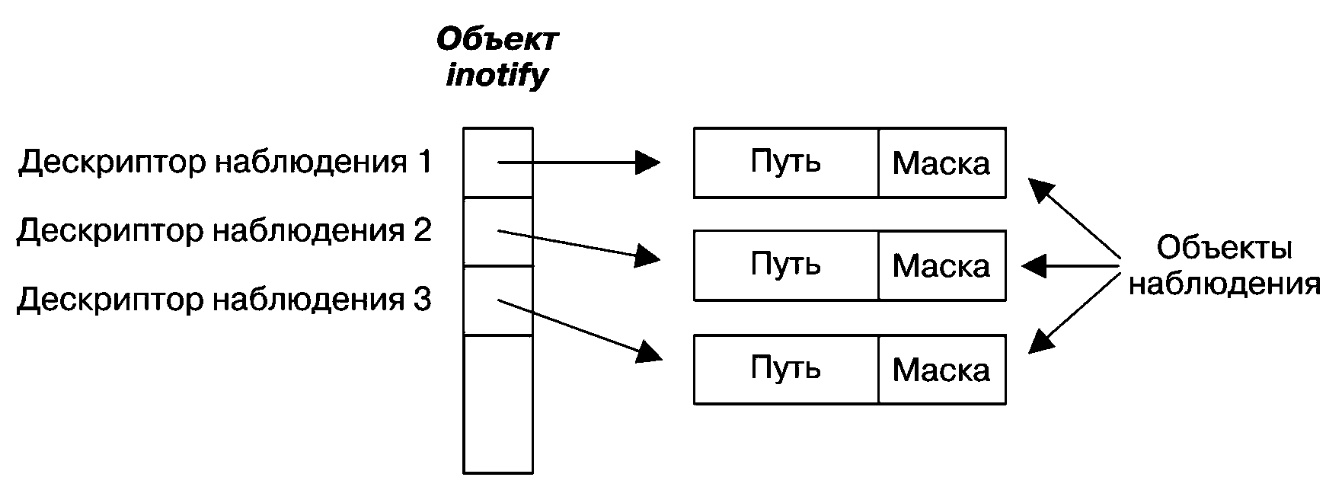
\includegraphics[width=.9\textwidth]{./imgs/inotify_object.png}
  \end{minipage}
  \caption{Объект inotify и связанные структуры данных ядра Linux.}
  \label{fig:inotify_object}
\end{figure}

Механизм inotify может использоваться для мониторинга файлов или каталогов. При
выполнении мониторинга в каталоге приложение будет проинформировано о событиях
для самого каталога и для файлов внутри каталога.

Механизм мониторинга inotify не является рекурсивным. Если приложение хочет
отслеживать события во всем поддереве каталогов, оно должно выполнять вызовы
\code{inotify\_add\_watch()} для каждого каталога в дереве.

Файловый дескриптор inotify можно читать с помощью \code{select()},
\code{poll()}, \code{epoll} и, начиная с Linux 2.6.25, механизмом ввода-вывода
на основе сигналов.

При добавлении экземпляра отслеживания аргумент \code{mask} определяет типы
событий, чей мониторинг должен осуществляться для указанного пути. Биты,
задающие эти типы приведены в таблице \ref{table:mask-in}.

\begin{table}[htb]
  \caption{\centering События inotify.}
  \small
  \centering\begin{tabular}{|l|l|}
              \hline\hline
              \multirow{ 2}{*}{Битовое значение} & \multirow{ 2}{*}{Описание}\\
                                                 & \\
              \hline
              \code{IN\_ACCESS} & Файл прочитан\\
              \hline
              \code{IN\_ATTRIB} & Метаданные изменены\\
              \hline
              \code{IN\_CLOSE\_WRITE} & Открытый для записи файл был закрыт \\
              \hline
              \code{IN\_CLOSE\_NOWRITE} & Открытый для чтения файл был закрыт \\
              \hline
              \code{IN\_CREATE} & Файл или каталог создан внутри наблюдаемого объекта \\
              \hline
              \code{IN\_DELETE} & Файл или каталог удален из наблюдаемого объекта \\
              \hline
              \code{IN\_DELETE\_SELF} & Наблюдаемый каталог или файл был удален \\
              \hline
              \code{IN\_MODIFY} & Файл был изменен \\
              \hline
              \code{IN\_MOVE\_SELF} & Наблюдаемый каталог или файл был перемещен \\
              \hline
              \code{IN\_MOVED\_FROM} & Файл или каталог перемещен из наблюдаемого каталога \\
              \hline
              \code{IN\_MOVED\_TO} & Файл или каталог перемещен в наблюдаемый каталог \\
              \hline
              \code{IN\_OPEN} & Файл был открыт \\
              \hline
              \code{IN\_ALL\_EVENTS} & Маска, содержащая все вышеперечисленные фильтры \\
              \hline
              \code{IN\_MOVE} & \code{IN\_MOVED\_FROM}|\code{IN\_MOVED\_TO} \\
              \hline
              \code{IN\_CLOSE} & \code{IN\_CLOSE\_WRITE}|\code{IN\_CLOSE\_NOWRITE} \\
              \hline
              \code{IN\_DONT\_FOLLOW} & Не разыменовывать символьные ссылки \\
              \hline
              \code{IN\_MASK\_ADD} & Добавить биты в текущую маску \\
              \hline
              \code{IN\_ONESHOT} & Отписаться после первого события \\
              \hline
              \code{IN\_ONLYDIR} & Возвращать ошибку, если переданный путь не является каталогом \\
              \hline\hline
            \end{tabular}
            \label{table:mask-in}
\end{table}


Зарегистрировав элементы в списке наблюдения, приложение может определить, какие
события произошли, используя \code{read()} для чтения событий из дескриптора
файла inotify. Если до сих пор не произошло никаких событий, то read()
блокируется.

После того, как произошли события, функция read() возвращает буфер, схема
которого представлена на рисунке \ref{fig:inotify_buffer}, содержащий одну или
несколько структур из листинга \ref{lst:inotify_event}.

\begin{listing}[H]
\caption{Структура \code{inotify\_event}}
\label{lst:inotify_event}
\begin{minted}[frame=single,fontsize = \footnotesize, linenos, xleftmargin = 1.5em]{c}
struct inotify_event {
    int wd;
    uint32_t mask;
    uint32_t cookie;
    uint32_t len;
    char[] name;
};
\end{minted}
\end{listing}

\begin{figure}[H]
  \centering
  \begin{minipage}[t]{.9\textwidth}
    \centering
    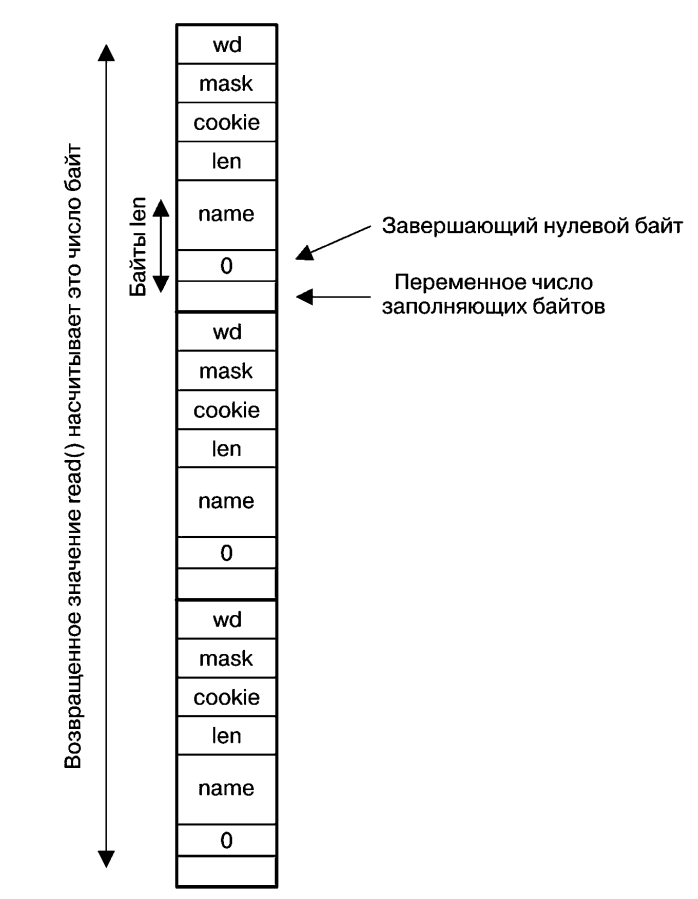
\includegraphics[width=.9\textwidth]{./imgs/inotify_buffer.png}
  \end{minipage}
  \caption{Буфер структур \code{inotify\_event.}}
  \label{fig:inotify_buffer}
\end{figure}

Поле wd содержит дескриптор наблюдения, для которого произошло это событие. Поле
wd полезно, когда приложение отслеживает несколько файлов или каталогов через
один и тот же файловый дескриптор inotify. Он предоставляет ссылку, которая
позволяет приложению определить конкретный файл или каталог, для которого
произошло событие. (Чтобы сделать это, приложение должно поддерживать кэш,
который связывает дескрипторы наблюдения с именами путей.)

Поле mask возвращает битовую маску, описывающую событие.

Поле cookie используется для связывания событий. В настоящее время это поле
используется только при переименовании файла. Когда это происходит, для
каталога, из которого переименован файл, генерируется событие
\code{IN\_MOVED\_FROM}, а затем для каталога, в который переименован файл,
генерируется событие \code{IN\_MOVED\_TO}. (Если файлу присваивается новое имя в
пределах одного и того же каталога, то оба события происходят для одного и того
же каталога.) Эти два события будут иметь одинаковое уникальное значение в поле
cookie, что позволит приложению связать их.

Когда происходит событие для файла в отслеживаемом каталоге, поле \code{name}
используется для возврата завершающейся нулем строки, идентифицирующей файл.
Если событие происходит для самого отслеживаемого объекта, то поле name не
используется, а поле \code{len} будет содержать 0.

Поле len указывает, сколько байт фактически выделено для поля \code{name}. Это
поле необходимо, поскольку между концом строки, сохраненной в \code{name}, и
началом следующей структуры \code{inotify\_event}, содержащейся в буфере,
возвращаемом \code{read()}, могут быть дополнительные пустые байты. Таким
образом, длина отдельного события inotify равна \code{sizeof(struct
  inotify\_event) + len}. Для хранения хотя бы одного события: буфер,
предоставленный для \code{read()} должен быть не менее \code{(sizeof(struct
  inotify\_event) + NAME\_MAX + 1)} байт, где \code{NAME\_MAX} --- это максимальная
длина имени файла плюс единица для завершающего нулевого байта.

Для хранения событий inotify в очереди используется память ядра. По этой причине
накладываются различные ограничения на работу механизма inotify. Администратор
может настроить эти ограничения с помощью трех файлов в каталоге
\code{/proc/sys/fs/inotify}:

\begin{itemize}
  \item \code{max\_queued\_events}. При вызове \code{inotify\_init()} это
        значение используется для установки верхнего предела для количество
        событий, которые могут быть поставлены в очередь для нового экземпляра
        inotify. Если это ограничение достигнуто, генерируется событие
        \code{IN\_Q\_OVERFLOW} и избыточные события отбрасываются. Поле
        \code{wd} для события переполнения будет иметь значение -1.
  \item \code{max\_user\_instances}. Это ограничение на количество экземпляров
        inotify, которые могут быть созданы для каждого реального пользователя
        системы.
  \item \code{max\_user\_watches}. Это ограничение на количество элементов
        просмотра, которые могут быть созданы для каждого реального пользователя
\end{itemize}

Типичные значения по умолчанию для этих трех файлов --- 16384, 128 и 8192
соответственно.

\subsection{fanotify}

Помимо описанных выше механизмов, в ядре Linux существует интерфейс <<fanotify>>
\cite{fanotify}. Он схож с inotify, но создан специально для поддержки
антивирусов.

\section{Разработка библиотеки}

Приложение будет являться клиентской библиотекой, предоставляющей интерфейс для
отслеживания событий файловой системы. Поддержка со стороны операционной системы
будет осуществляться с помощью одного из механизмов, описанных выше. Библиотека
должна будет иметь функции для рекурсивного отслеживания иерархии подкаталогов и
преобразовывать события в удобный для пользователей формат.

Для получения событий от операционной системы выбран механизм inotify, так как
он является самым гибким и актуальным, среди изложенных выше способов. Кроме
того, в контексте операционной системы Linux, чаще всего возникают основные
сценарии применения inotify.

% В конструкторском разделе на основе сделанного во
% введении обзора проводится обоснованный выбор предлагаемого алгоритма, подробно
% описывается его использование применительно к решаемой задаче. Также
% производится проектирование архитектуры и модулей разрабатываемого приложения
% или пакета программ, интерфейсов их взаимодействия, определяются форматы
% представления входных и выходных данных, разрабатываются структуры данных для их
% внутреннего представления. В данном разделе расчётно-пояснительной записки могут
% выполняться рас¬четы для определения объемов памяти, необходимой для хранения
% исходных данных, промежуточных и окончательных результатов, а также расчеты,
% позволяющие оценить теоретическую сложность реализуемых алгоритмов.

\subsection{Выбор инструментов разработки}

Для разработки библиотеки был выбран язык Go из-за следующих его особенностей:

\begin{enumerate}
	\item Отсутствие библиотек, соответствующих заявленным требованиям к
        библиотеке в рамках данной работы;
	\item Наличие кодогенерированных нативных функций, реализующих интерфейс
        системных вызовов inotify;
	\item Поддержка конкурентного выполнения кода в базовой поставке языка \cite{effectivego};
  \item Схожесть с языком C, простота написания кода, минималистичность.
\end{enumerate}

При написании библиотеки использовался Go версии \code{1.21.6}.

Список внешних зависимостей небольшой:

\begin{enumerate}
  \item \code{github.com/google/uuid v1.6.0}~\cite{uuid}. Используется для генерации
        уникальных идентификаторов для экземпляров inotify.
  \item \code{github.com/stretchr/testify v1.8.4}~\cite{testify}. Используется для удобного
        написания unit и end-to-end тестов.
  \item \code{golang.org/x/sys v0.17.0}~\cite{golangunix}. Подключает системные вызовы
        операционной системы Linux.
\end{enumerate}

Из пакетов стандартной библиотеки можно выделить \code{log/slog}. Это
современный интерфейс для структурного логирования.

\subsection{Архитектура библиотеки}

Библиотека должна состоять из одного компонента --- структуры <<Наблюдатель>>.
Эта структура инкапсулирует в себе состояние экземпляра inotify, предоставялет
возможность подписываться на события каталога или файла, читать события и
прекращать получение событий файловой системы.

\subsection{Разработка моделей библиотеки}

Для эффективного использования библиотеки необходимо разработать две ключевые
модели --- модель <<Наблюдатель>> и модель <<Событие>>. Эти модели играют
центральную роль в интерфейсе библиотеки, и используются при преобразовании
<<сырых>> событий файловой системы, к удобным для пользователя событиям.

Модель <<Событие>> представляет собой одно или несколько событий,
сгенерированных inotify.

Поля модели события:

\begin{itemize}
	\item Путь
	\item Флаг директории
  \item Тип события
  \item Другие специфичные для данного события поля
\end{itemize}

Модель <<Наблюдатель>> реализует функционал:

\begin{itemize}
  \item Подписка на события каталога
  \item Рекурсивная подписка на события иерархии подкаталогов
  \item Отписка от событий каталоги или иерархии подкаталогов
  \item Чтение событий
  \item Остановка чтения событий
\end{itemize}

Разработанные модели обеспечивают необходимый фундамент для эффективной работы
пользовательского кода с событиями файловой системы. Модель события обеспечивает
удобное представление информации о любой операции над файлами или каталогами.

\subsection{Применение inotify}

В рамках разрабатываемой библиотеки, основным способом получения событий
файловой системы будет являться механизм inotify. Структура <<Наблюдатель>>
инкапсулирует работу с системными вызовами.

Для чистоты интерфейса необходимо реализовать кэширование соответствия
дескрипторов наблюдения с отслеживаемыми путями. При удалении отслеживаемой
директории, удалять соответствия из хэш-таблицы, а при добавлении, вставлять в
нее новые значения.

Также нужно реализовать объединение нескольких событий inotify в одно, для
поддержки событий переименования (перемещения), а так же для избежания
дублирования событий при удалении отслеживаемого каталога внутри другого
отслеживаемого каталога.

Для реализации рекурсивного отслеживания иерархии подкаталогов файловой системы,
помимо кэширования соответствия дескрипторов, необходимо реализовать рекурсивный
обход новых папок, после их добавления в список отслеживаемых, с последующей
генерацией нужных событий для пользовательского кода. Это не позволит избежать
большинства состояний гонки, но будет приводить систему в консистентное
сосотояние, от чего напрямую зависит надежность библиотеки.

Как отмечалось выше, пара событий \code{IN\_MOVED\_FROM} и \code{IN\_MOVED\_TO},
сгенерированная \code{rename()}, может быть сопоставлена с помощью их общего
значения cookie. Однако задача сопоставления сопряжена с некоторыми трудностями.

Эти два события обычно следуют друг за другом в потоке событий, доступном при
чтении из файлового дескриптора inotify. Однако это не гарантируется
(гарантируется, что \code{IN\_MOVED\_FROM} приходит всегда раньше
\code{IN\_MOVED\_TO}, так как очередь событий упорядоченная). Если несколько
процессов запускают события для отслеживаемых объектов, то (в редких случаях)
между событиями может появиться произвольное количество других событий Кроме
того, не гарантируется, что пара событий атомарно вставлена в очередь: может
быть короткий интервал, когда \code{IN\_MOVED\_FROM} появился, а
\code{IN\_MOVED\_TO} --- нет.

Таким образом, сопоставление пары событий \code{IN\_MOVED\_FROM} и
\code{IN\_MOVED\_TO}, сгенерированных \code{rename} уязвимо для ошибок.
(Например, если объект переименован за пределами отслеживаемого каталога,
события \code{IN\_MOVED\_TO} может даже не произойти.) Эвристические подходы
(например, предположим, что события всегда следуют друг за другом) могут быть
использованы для обеспечения совпадения в большинстве случаев, но неизбежно
приведут к ошибкам, когда приложение воспринимает события \code{IN\_MOVED\_FROM}
и \code{IN\_MOVED\_TO} как не связанные. Если в результате дескрипторы наблюдения будут
уничтожены и созданы заново, то эти дескрипторы наблюдения будут несовместимы с
дескрипторами наблюдения в любых ожидающих событиях. (Повторное создание
дескриптора inotify и перестройка кэша могут помочь.)

Приложения также должны допускать возможность того, что событие
\code{IN\_MOVED\_FROM} было последним событием, которое могло поместиться в
буфер, возвращаемый текущим вызовом \code{read()}, и сопутствующее событие
\code{IN\_MOVED\_TO} может быть извлечено только при следующем чтении, что
должно быть сделано с (небольшим) тайм-аутом, чтобы учесть тот факт, что вставка
пары событий \code{IN\_MOVED\_FROM+IN\_MOVED\_TO} не является атомарной, а также
возможность того, что может не быть никакого события \code{IN\_MOVED\_TO}.

В таблице~\ref{table:mask-out} приведем возможные значения маски для
сгенерированных событий.

\begin{table}[htb]
  \caption{\centering События inotify.}
  \small
  \centering\begin{tabular}{|l|l|}
              \hline\hline
              \multirow{ 2}{*}{Битовое значение} & \multirow{ 2}{*}{Описание}\\
                                                 & \\
              \hline
              \code{IN\_ACCESS} & Файл прочитан\\
              \hline
              \code{IN\_ATTRIB} & Метаданные изменены\\
              \hline
              \code{IN\_CLOSE\_WRITE} & Открытый для записи файл был закрыт \\
              \hline
              \code{IN\_CLOSE\_NOWRITE} & Открытый для чтения файл был закрыт \\
              \hline
              \code{IN\_CREATE} & Файл или каталог создан внутри наблюдаемого объекта \\
              \hline
              \code{IN\_DELETE} & Файл или каталог удален из наблюдаемого объекта \\
              \hline
              \code{IN\_DELETE\_SELF} & Наблюдаемый каталог или файл был удален \\
              \hline
              \code{IN\_MODIFY} & Файл был изменен \\
              \hline
              \code{IN\_MOVE\_SELF} & Наблюдаемый каталог или файл был перемещен \\
              \hline
              \code{IN\_MOVED\_FROM} & Файл или каталог перемещен из наблюдаемого каталога \\
              \hline
              \code{IN\_MOVED\_TO} & Файл или каталог перемещен в наблюдаемый каталог \\
              \hline
              \code{IN\_OPEN} & Файл был открыт \\
              \hline
              \code{IN\_IGNORED} & Файл более не отслеживается\\
              \hline
              \code{IN\_ISDIR} & Событие относится к каталогу\\
              \hline
              \code{IN\_Q\_OVERFLOW} & Переполнение очереди событий\\
              \hline
              \code{IN\_UNMOUNT} & Файловая система была размонтирована\\
              \hline\hline
            \end{tabular}
            \label{table:mask-in}
\end{table}

Предположим, приложение отслеживает каталог dir и файл dir/myfile для всех
событий. В листинге \ref{lst:inotify_examples} ниже показаны некоторые события, которые будут сгенерированы
для этих двух объектов.

\begin{listing}[H]
\caption{Примеры событий inotify}
\label{lst:inotify_examples}
\begin{minted}[frame=single,fontsize = \footnotesize, linenos, xleftmargin = 1.5em]{c}
fd = open("dir/myfile", O_RDWR);
// Генерирует события IN_OPEN как для dir, так и для dir/myfile.

read(fd, buf, count);
// Генерирует события IN_ACCESS как для dir, так и
// для dir/myfile.

write(fd, buf, count);
// Генерирует события IN_MODIFY как для dir, так и
// для dir/myfile.

fchmod(fd, mode);
// Генерирует события IN_ATTRIB как для dir, так и
// для dir/myfile.

close(fd);
//Генерирует события IN_CLOSE_WRITE как для dir,
// так и для dir/myfile.
\end{minted}
\end{listing}


Предположим, приложение просматривает каталоги dir1 и dir2,
и файл dir1/myfile. В листинге \ref{lst:inotify_examples2} показаны некоторые
события, которые могут быть сгенерированы.

\begin{listing}[H]
\caption{Примеры событий inotify}
\label{lst:inotify_examples2}
\begin{minted}[frame=single,fontsize = \footnotesize, linenos, xleftmargin = 1.5em]{c}
link("dir1/myfile", "dir2/new");
// Генерирует событие IN_ATTRIB для myfile и
// событие IN_CREATE для dir2.

rename("dir1/myfile", "dir2/myfile");
// Генерирует событие IN_MOVED_FROM для dir1,
// событие IN_MOVED_TO для dir2 и событие IN_MOVE_SELF
//      для myfile. События IN_MOVED_FROM и IN_MOVED_TO
//      будут иметь одинаковое значение cookie.
\end{minted}
\end{listing}

Предположим, что dir1/xx и dir2/yy являются (единственными) ссылками на один и
тот же файл, и приложение просматривает dir1, dir2, dir1/xx и dir2/yy. Выполняя
следующие вызовы в порядке, указанном в листинге \ref{lst:inotify_examples3}
сгенерируются следующие события:

\begin{listing}[H]
\caption{Примеры событий inotify}
\label{lst:inotify_examples3}
\begin{minted}[frame=single,fontsize = \footnotesize, linenos, xleftmargin = 1.5em]{c}
unlink("dir2/yy");
// Генерирует событие IN_ATTRIB для xx (поскольку изменяется его ссылка
// count) и событие IN_DELETE для dir2.

unlink("dir1/xx");
// Генерирует события IN_ATTRIB, IN_DELETE_SELF и IN_IGNORED
// для xx и событие IN_DELETE для dir1.
\end{minted}
\end{listing}

Предположим, приложение просматривает каталог dir и (пустой) каталог dir/subdir.
В следующих примерах в листинге \ref{lst:inotify_examples4} показаны некоторые события, которые могут быть
сгенерированы.

\begin{listing}[H]
\caption{Примеры событий inotify}
\label{lst:inotify_examples4}
\begin{minted}[frame=single,fontsize = \footnotesize, linenos, xleftmargin = 1.5em]{c}
mkdir("dir/new", mode);
// Генерирует событие IN_CREATE | IN_ISDIR для dir.

rmdir("dir/subdir");
// Генерирует события IN_DELETE_SELF и IN_IGNORED для
// subdir и событие IN_DELETE | IN_EDIT для dir.
\end{minted}
\end{listing}

\subsection{Проектирование интерфейса}

У модели <<Наблюдатель>> спроектированы следующие методы:

\begin{itemize}
  \item \code{NewWatch(chan)} --- конструктор. На вход принимает буфер
        \code{chan}, куда будут записываться генерируемые события;
  \item \code{Subscribe(path string)} --- функция подписки на путь. Создает
        дескриптор наблюдения, по завершению вызова в буфер начинают
        записываться события по этому пути. Путь может быть файлом или
        директорией;
  \item \code{Unsubscribe(path string)} --- функция прекращения отслеживания пути.
  \item \code{SubscrubeRecursive(path string)} --- функция рекурсивной подписки
        на иерархию подкаталогов каталога \code{path};
  \item \code{Close()} --- функция прекращающая отправку событий по всем
        десприпторам наблюдения.
\end{itemize}

Функции Subscribe и SubscribeRecursive покрывают почти все сценарии использования
inotify. При применении SubscribeRecursive созданные подкаталоги автоматически
попадают в список отслеживаемых.

Из непокрытых сценариев использования, могут быть сценарии, когда необходимо
исключить некоторые подкаталоги с помощью фильтров по регулярным выражениям.
Кроме того, отписка от уведомлений не имеет рекурсивной версии.

Данный набор методов удовлетворяет требованиям к сущности <<Наблюдатель>>,
инкапсулируют логику чтения событий с помощью механизма inotify и предоставляет
удобный интерфейс для пользователей.

\section{Реализация библиотеки}

% Технологический раздел должен содержать обоснование выбранных для реализации
% комплекса программ языков программирования, технологий и сторонних библиотек.
% Для полноты изложения приводятся ключевые моменты программной реализации
% разрабатываемых программ. В технологический раздел также включаются
% руководство администратора и руководство пользователя. Руководство
% администратора должно включать описание процедуры инсталляции и деинсталляции
% приложения, параметры запуска из командной строки, перечень требований к
% аппаратному и системному программному обеспечению, наличию каких-либо
% сторонних приложений или библиотек. Руководство пользователя должно содержать
% подробное описание графического и/или командного интерфейса разработанного
% приложения, перечень сообщений об ошибках с их описанием. В случае разработки
% библиотеки функций, а не пользовательского или системного приложения,
% руководство пользователя заменяется на описание программного интерфейса (API)
% библиотеки.

Для выполнения поставленной задачи необходимо реализовать структуру
<<Наблюдатель>>, инкапсулирующую работу с системным интерфейсом inotify.

Разработка проекта осуществлялась в редакторе Emacs. Данный редактор может быть
использван в качестве IDE благодаря обширной библиотеке расширений. Для
конфигурирования редактора использован фреймворк Doom Emacs, в стандартной
поставке которого настроены инструменты для рефакторинга и анализа кода на Go,
необходимые для удобной и эффективной рабзработки.

Для настройки рабочего окружения использована связка менеджера пакетов
\code{Nix} и утилиты для настройки локальных окружений \code{lorri}. Это
позволяет декларативно описывать воспроизводимые окружения разработки и сборки
приложений и библиотек.

Для сборки кода и тестов используется утилита \code{go} из стандартной поставки
языка программирования \code{Go}.

\subsection{Особенности реализации модуля <<Наблюдатель>>}

Структура <<Наблюдатель>> хранит состояние чтения событий из интерфейса inotify,
а так же кэширует соответствие дескрипторов наблюдения и путей файловой системы.
Объявление структуры приведено в листинге \ref{lst:watcher}.

\begin{listing}[H]
\caption{Структура Watch}
\label{lst:watcher}
\begin{minted}[frame=single,fontsize = \footnotesize, linenos, xleftmargin = 1.5em]{c}
type Watch struct {
	events chan<- Event
	logger *slog.Logger

	inotify *os.File
	buf *inotifyBuffer
	nameByWatchDescriptor map[int] string

	stopServing chan<- struct{}
}
\end{minted}
\end{listing}

Как видно на листинге \ref{lst:watcher}, библиотека использует канал \code{events} для передачи
событий пользовательскому коду. Поля \code{inotify}, \code{buf} и
\code{nameByWatchDescriptor} отвечают за взаимодействие с API intofify. Канал
\code{stopServing} используется для остановки чтения и отправки эвентов
пользовательскому коду.

На листинге \ref{lst:newwatch} отображен код конструктора структуры <<Наблюдатель>>.

\begin{listing}[H]
\caption{Конструктор NewWatch}
\label{lst:newwatch}
\begin{minted}[frame=single,fontsize = \footnotesize, linenos, xleftmargin = 1.5em, breaklines]{c}
func NewWatch(events chan<- Event, logger *slog.Logger) (Watch, error) {
	fd, err := unix.InotifyInit()

// ...

	stopServing := make(chan struct{})

//...

	logger.Info("Initialized new inotify instance", "inotify", w.inotify.Name())

	go w.serveEvents(stopServing)

	return w, nil
}
\end{minted}
\end{listing}

Как видно из листинга, конструктор инициализирует дескриптор inotify и запускает
горутину, которая вычитывает события из буфера inotify и отправляет в
пользовательский код через канал \code{events}.

Необходимо заметить, что канал в данном случае является частью публичного
интерфейса библиотеки, поэтому соответствует трем правилам проектирования таких интерфейсов~\cite{goapichannels}:

\begin{enumerate}
  \item Указывать направление канала.
  \item Получать канал как параметр. Тогда пользовательский код может без
        проблем настраивать наличие и размер буфера.
  \item Закрывать такой канал может только горутина, записывающая значения.
\end{enumerate}

Рассмотрим функцию подписки на путь в листинге~\ref{lst:subscribe}. Функция
принимет на вход путь. Затем создает новый дескриптор наблюдения и кэширует
соответствие этого дескриптора с переданным путем.

\begin{listing}[H]
\caption{Функция подписки на события}
\label{lst:subscribe}
\begin{minted}[frame=single,fontsize = \footnotesize, linenos, xleftmargin = 1.5em, breaklines]{c}
func (w *Watch) Subscribe(path string) error {
	wd, err := unix.InotifyAddWatch(int(w.inotify.Fd()), path, unix.IN_ALL_EVENTS)
	if err != nil {
		return err
	}
	w.nameByWatchDescriptor[wd] = path
	w.logger.Info("Subscribed to new path", "wd", wd, "path", path)
	return nil
}
\end{minted}
\end{listing}

Объявления типов событий приведено в листинге~\ref{lst:event}. Здесь
\code{Event} имеет тип \code{any}, что подразумевает определение типа события с
помощью type switch в пользовательском коде, пример в листинге~\ref{lst:typeswitch}.

\begin{listing}[H]
\caption{Объявления типов событий}
\label{lst:event}
\begin{minted}[frame=single,fontsize = \footnotesize, linenos, xleftmargin = 1.5em, breaklines]{c}
type Event any

type CreateEvent struct {
	Path string
	IsDir bool
}

type DeleteEvent struct {
	Path string
	IsDir bool
}

type RenameEvent struct {
	Path string
	IsDir bool
	MovedTo string
}

// ...

\end{minted}
\end{listing}

\begin{listing}[H]
\caption{Пример определение типа события}
\label{lst:typeswitch}
\begin{minted}[frame=single,fontsize = \footnotesize, linenos, xleftmargin = 1.5em, breaklines]{c}
	select {
	case e := <-events:
		switch e := e.(type) {
		case inotify.CreateEvent:
			fmt.Println("create ", e.Path)
    // ...
		}
	case <-time.After(1*time.Second):
		os.Exit(1)
	}
\end{minted}
\end{listing}

В листинге~\ref{lst:serve} приведен код горутины, которая читает обновления
inotify и отправляет пользовательскому коду.

\begin{listing}[H]
\caption{Горутина, читающая события и направляющая пользовательскому коду}
\label{lst:serve}
\begin{minted}[frame=single,fontsize = \footnotesize, linenos, xleftmargin = 1.5em, breaklines]{c}
func (w *Watch) serveEvents(stop <-chan struct{}) {
	defer w.logger.Info("Stop serving events", "inotify", w.inotify.Name())
	w.logger.Info("Start serving events", "inotify", w.inotify.Name())
	for {
		event, err := w.readEvent()
		if err != nil {
			w.logger.Warn(fmt.Sprintf("Got error while reading events: %v", err.Error()))
			close(w.events)
			return
		}
		select {
		case w.events <- w.convertToEvent(event):
			w.logger.Debug("Serve event", "value", event)
		case <-stop:
			w.logger.Debug("serveEvents got stop signal")
			close(w.events)
			return
		}
	}
}
\end{minted}
\end{listing}

Интересно рассмотреть функцию прекращения мониторинга в
листинге~\ref{lst:close}. Т.к. чтение событий и запись в канал происходит в
отдельной горутине, если не предпринять специальных мер, при уничтожении объекта
\code{Watch}, эта горутина останется в заснувшем состоянии, потребляя ресурсы
системы. Для нормального завершения работы нужно всегда вызывать функцию
\code{Close()} после окончания обработки событий. Эта функция остановит горутину одним из двух способов:

\begin{itemize}
  \item Если горутина заблокировалась на чтении из файлового дескриптора
        inotify, то \code{Close()} закроет этот файловый дескриптор, и горутина
        разблокируется.
  \item Если горутина заблокировалась на записи в канал, то \code{Close()}
        закроет канал \code{stopServing}, и горутина также разблокируется.
\end{itemize}

Таким образом все ресурсы корректно освобождаются в конце чтения событий.

\begin{listing}[H]
\caption{Функция остановки получения событий.}
\label{lst:close}
\begin{minted}[frame=single,fontsize = \footnotesize, linenos, xleftmargin = 1.5em, breaklines]{c}
func (w *Watch) Close() {
	close(w.stopServing)
	w.inotify.Close()
}
\end{minted}
\end{listing}

\subsection{Описание работы библиотеки}

В листинге~\ref{lst:logger_code} приведен пример использования библиотеки. Последовательность действий:

\begin{enumerate}
  \item Создать канал для событий.
  \item Вызвать конструктор NewWatch и передать канал туда.
  \item Сделать отложенный вызов Close.
  \item Подписаться на нужные каталоги.
  \item Читать события из канала.
\end{enumerate}

Запуск приложения производиться согласно рисунку \ref{fig:run_app}. Зависимости
устанавливаются утилитой \code{go} автоматически. После успешной сборки в
консоли будут логироваться события.

\begin{figure}[H]
	\centering
	\begin{minipage}[t]{.8\textwidth}
		\centering
		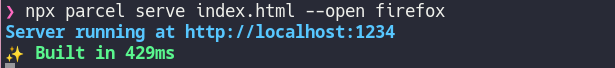
\includegraphics[width=.8\textwidth]{./imgs/run_app.png}
	\end{minipage}
	\caption{Пример запуска приложения.}
	\label{fig:run_app}
\end{figure}

\section{Тестирование}

Для тестирования приложения проведем серию тестов, где выполним некоторые
операции над файлами внутри наблюдаемых каталогов и сравним полученные события с
ожидаемыми.

Для каждого теста ниже, в начале производится одинаковая настройка окружения.
Приведено в лисинге~\ref{lst:test_setup}.

\begin{listing}[H]
\caption{Настройка тестового окружения}
\label{lst:test_setup}
\begin{minted}[frame=single,fontsize = \footnotesize, linenos, xleftmargin = 1.5em, breaklines]{c}
func (s *InotifyTestSuite) SetupTest() {
	root, err := os.MkdirTemp("", "inotify-go")
	if err != nil {
		panic(err)
	}
	s.root = root
	h := slog.NewTextHandler(os.Stderr, &slog.HandlerOptions{Level: slog.LevelDebug})
	slog.SetDefault(slog.New(h))
}

func (s *InotifyTestSuite) TearDownTest() {
	err := os.Remove(s.root)
	if err != nil {
		panic(err)
	}
}
\end{minted}
\end{listing}

В листинге~\ref{lst:test_create} приведен юнит-тест, где проверяется отправка
события создания файла в наблюдаемом каталоге.

\begin{listing}[H]
\caption{Тест на создание файла}
\label{lst:test_create}
\begin{minted}[frame=single,fontsize = \footnotesize, linenos, xleftmargin = 1.5em, breaklines]{c}
func (s *InotifyTestSuite) TestServeFileCreateEvent() {
	events := make(chan Event)
	w, _ := NewWatch(events, slog.Default())
	defer w.Close()
	w.Subscribe(s.root)
	path := filepath.Join(s.root, "test")
	file, _ := os.Create(path)
	defer os.Remove(file.Name())
	file.Close()

	event := <-events

	require.Equal(s.T(), CreateEvent{
		Path:  file.Name(),
		IsDir: false,
	}, event)
}
\end{minted}
\end{listing}

В листинге~\ref{lst:test_delete} приведен юнит-тест, где проверяется отправка
события удаления файла в наблюдаемом каталоге.

\begin{listing}[H]
\caption{Тест на удаление файла}
\label{lst:test_delete}
\begin{minted}[frame=single,fontsize = \footnotesize, linenos, xleftmargin = 1.5em, breaklines]{c}
func (s *InotifyTestSuite) TestServeFileDeleteEvent() {
	events := make(chan Event)
	w, _ := NewWatch(events, slog.Default())
	defer w.Close()
	file, _ := os.CreateTemp(s.root, "test")
	file.Close()
	w.Subscribe(s.root)

	os.Remove(file.Name())
	event := <-events

	require.Equal(s.T(), DeleteEvent{
		Path:  file.Name(),
		IsDir: false,
	}, event)
}
\end{minted}
\end{listing}

В листинге~\ref{lst:test_delete} приведен юнит-тест, где проверяется отправка
события удаления наблюдаемого каталога.

\begin{listing}[H]
\caption{Тест на удаление каталога}
\label{lst:test_delete_self}
\begin{minted}[frame=single,fontsize = \footnotesize, linenos, xleftmargin = 1.5em, breaklines]{c}
func (s *InotifyTestSuite) TestServeDeleteSelfEvent() {
	events := make(chan Event)
	w, _ := NewWatch(events, slog.Default())
	defer w.Close()
	dir, _ := os.MkdirTemp(s.root, "test")
	w.Subscribe(s.root)
	w.Subscribe(dir)

	os.Remove(dir)
	event := <-events

	require.Equal(s.T(), DeleteEvent{
		Path:  dir,
		IsDir: true,
	}, event)
}
\end{minted}
\end{listing}

Аналогичные тесты сделаны и для других типов событий. На последней версии
библиотеки все тесты завершаются успехом.

\subsection{Результаты тестирования}

В результате тестирования библиотеки на различных видах операций над файлами и
сравнения полученных событий с ожидаемыми, можно утверждать о правильности
работы библиотеки. Программа показала согласованность и точность в уведомлении о
событиях файловой системы для разнообразных входных данных, включая создание,
переименование, удаление и т.д. На каждом этапе тестирования результирующий
список событий совпадал с ожидаемым.

Таким образом, результаты тестирования позволяют сделать вывод о правильности
работы разработанной библиотеки и её способности генерировать уведомления об
операциях над файлами и каталогами в различных сценариях использования.

\newpage
\anonsection{ЗАКЛЮЧЕНИЕ}  %Заключение

В ходе выполнения курсовой работы был проведен анализ способов получения событий
файловой системы в операционной системе Linux. Рассмотрены различные механизмы,
предоставляемые ядром для этих целей. Изучены их сильные и слабые стороны,
области применения.

Основной целью данной курсовой работы была реализация библиотеки для уведомления
об операциях над файлами и каталогами. Результаты выполнения задачи
демонстрируют удовлетворительное качество работы библиотеки, что подтверждается
сравнением с ожидаемыми резульататми на разнообразных входных данных.
Разработанное программное решение представляет собой инструмент для гибкого и
удобного получения событий файловой системы в среде операцинной системы Linux.

В заключение, несмотря на достигнутые положительные результаты, существует
потенциал для дальнейшего улучшения программы. Это включает в себя оптимизацию
механизмов обработки и анализа событий, адаптацию программы для использования
других механизмов получения событий, а также улучшения интерфейса.

\renewcommand\refname{СПИСОК ИСПОЛЬЗОВАННЫХ ИСТОЧНИКОВ}
% Список литературы
\clearpage
%\bibliographystyle{ugost2008s}  %utf8gost71u.bst} %utf8gost705u} %gost2008s}
{\catcode`"\active\def"{\relax}
\addcontentsline{toc}{section}{\protect\numberline{}\refname}%
%\bibliography{biblio} %здесь ничего не меняем, кроме, возможно, имени bib-файла
\printbibliography
}
\newpage
\settocdepth{section}
\anonsection{ПРИЛОЖЕНИЕ А}
\vspace{-30pt}

\begin{listing}[H]
\caption{Пример использования библиотеки.}
\label{lst:logger_code}
\begin{minted}[frame=single,fontsize = \footnotesize, linenos, xleftmargin = 1.5em, breaklines]{c}
package main

import (
	"fmt"
	"log/slog"
	"os"
	"time"

	"github.com/stewkk/iu9-coursework/pkg/inotify"
)

func main() {
	events := make(chan inotify.Event, 10)
	w, err := inotify.NewWatch(events, slog.Default())
	if err != nil {
		panic(err)
	}
	defer w.Close()
	select {
	case e := <-events:
		switch e := e.(type) {
		case inotify.CreateEvent:
			fmt.Println("create ", e.Path)
	    // ...
		}
	case <-time.After(1*time.Second):
		os.Exit(1)
	}
}
\end{minted}
\end{listing}

\end{document}
